\chapter{Post-Processing}
\label{post_processing}

Nachdem möglichst alle low-level Änderungen zu Semantic-Change-Sets (SCS)  gruppiert wurden, muss
die Differenz in einem weiteren Schritt optimiert werden. Bis hierhin ist es möglich, dass sich die
SCS in Teilen überschneiden oder sogar identisch sind. Im Folgenden wird jedes SCS als Menge
(\textit{engl. Set}) betrachtet. Eine low-level Änderung ist ein Element, aus der sich die Mengen
zusammensetzten. Ein Element kann in mehreren Mengen vorkommen, aber nur einmal in einer Menge. Zwei
SCS überschneiden sich also genau dann, wenn mindestens einmal die selbe low-level Änderung in
beiden SCS vorkommt. Zwei SCS sind identisch, wenn beide die selben low-level Änderungen enthalten.
Zu Beginn müssen die Kriterien festgelegt werden, nach denen die geliftete Differenz optimiert
werden soll:

\begin{enumerate}
  \item Eliminieren aller Überschneidungen von SCS. D.h. nach dem Post-Processing soll jede
  low-level Änderung nur in genau einem SCS vorkommen.
 
  \item Erreichen einer möglichst guten Abdeckung der low-level Änderungen. D.h. beim Entfernen von
  sich überschneidenden SCS sollen möglichst wenige bis keine low-level Änderungen entstehen, die in
  keinem SCS enthalten sind.

  \item \textbf{Kompression:} Es sollten möglichst die SCS mit großem Betrag ($|SCS|$) erhalten
  bleiben. D.h. ein SCS mit vielen low-level Änderungen wird gegenüber einem SCS mit wenigen
  Änderungen bevorzugt.
\end{enumerate}
Der im Folgenden vorgestellte Algorithmus ist in 5  Schritte aufgeteilt. Das Vorgehen basiert
auf dem in \cite{KeKT2011ASE} (S.8) beschriebenen Konzept. In jedem Schritt wird die Differenz nach
den oben beschriebenen Kriterien weiter optimiert. Um den Algorithmus zu notieren werden zwei neue
Mengen für SCS eingeführt.

\begin{itemize}
  \item $PCS_{min}$: In dieser Menge werden alle überschneidungsfreien SCS abgelegt, die später in
  der Differenz erhalten bleiben sollen.
 
  \item $PCS_D$: Diese Menge enthält die noch zu bearbeitenden SCS. $PCS_D$ enthält zu Beginn alle
  potenziellen SCS aus der gelifteten Differenz. Während jedem Schritt des Algorithmus wird $PCS_D$
  nach den oben beschriebenen Kriterien optimiert. D.h. alle SCS, die Überschneidungen aufweisen,
  werden nach und nach entfernt. Alle SCS, die überschneidungsfrei sind, werden dann aus $PCS_D$ in
  $PCS_{min}$ verschoben. Am Ende des Algorithmus muss $PCS_D$ leer sein.
\end{itemize}

\section{Identische Semantic Change Sets}

Zu Beginn wird $PCD_D$ mit allen potenziellen SCS aus der Differenz gefüllt. Identische SCS können
relativ leicht identifiziert werden und werden deshalb bereits hier ausgefiltert. Um zu entscheiden
welche SCS behalten werden sollen und welche verworfen werden, wurden zwei Qualitätskriterien für
SCS angelegt.

\begin{itemize}
  \item \textbf{Priority:} Die Priorität kann für jede Regel konfiguriert werden. Die Priorität wird
  als Integerwert angegeben. Eine hohe Priorität wird durch einen großen Wert angegeben, eine
  niedrige Priorität durch einen kleinen Wert. Es sind auch negative Werte möglich. Als Standard
  wird bei der Generierung der Wert 1 für normale Erkennungsregeln und 0 für Erkennungsregeln mit
  einer Amalgamation-Unit gesetzt. Am häufigsten tritt das Problem von identischen SCS dann auf,
  wenn nur die Kernregel einer Amalgamation-Unit Erkennungsregel ausgeführt wird und die Kernregel genau
  einer normalen Erkennungsregel entspricht. Zum Beispiel hat die Advanced-Regel Pull-Up-EAttribute
  als Kernregel die Atomic-Regel Move-EAttribute. In der Regel möchte man aber in einem Fall, wo nur
  ein einziges Attribut verschoben wurde, eher die Move Regel als die Pull-Up Regel als Lifting
  angezeigt bekommen.
 
  \item \textbf{Refinment-Level:} Wenn anhand der Priorität keine Entscheidung über die identischen
  SCS getroffen werden kann, weil beide Prioritäten ebenfalls gleich sind, wird das Refinment-Level
  betrachtet. Der Wert des Refinment-Level leitet sich aus der Editierregel ab und  gibt an wie
  speziell bzw. abstrakt eine Editierregel ist. Dazu wird für jeden (\texttt{<<delete>>},
  \texttt{<<create>> und \texttt{<<preserve>}}) Knoten der Edierregel die Anzahl der Supertypen
  ermittelt und aufsummiert. Dieser Wert wird direkt bei der Generierung der Erkennungsregel
  ermittelt und beim Ausführen der Erkennungsregel in das erzeugte SCS geschrieben. Im Sinne des
  Semantic-Liftings soll die möglichst spezielle Editieroperation angezeigt werden. Daher werden SCS
  mit einem hohen Refinment-Level bevorzugt in $PCD_D$ übernommen. Zum Beispiel die Editieroperation
  die das Attribut \texttt{name} der abstrakten Ecore Klasse \texttt{ENamedElement} setzt, hat ein
  Refinment-Level von 1, da der einzige Supertyp \texttt{EModelElement} ist. Im Gegensatz dazu hat
  die Editieroperation, die den in diesem Fall vererbten Namen einer \texttt{EClass} setzt, ein
  Refinment-Level von 3. Die Supertypen sind hier: \texttt{EClassifier}, \texttt{ENamedElement} und
  \texttt{EModelElement}.
\end{itemize}
Ist auch das Refinment-Level der SCS gleich, so wird das erste in Differenz vorkommende SCS in
$PCD_D$ übernommen. Das Resultat dürfte allerdings relativ zufällig sein, da die SCS parallel
berechnet wurden. Außerdem wurden in verschiedenen Berechnungsschritten zuvor Sets verwendet, die
auf Hashfunktionen basieren. Daher ist die Reihenfolge der SCS in der Differenz nicht abzusehen.

\section{Überschneidungsfreie Semantic Change Sets}

Alle SCS die keine Überschneidungen mit anderen SCS haben, können sofort aus $PCS_D$ in $PCS_{min}$
verschoben werden. In der Praxis dürften in der Regel die meisten SCS überschneidungsfrei sein. Nach
Definition im Abschnitt \ref{editierregeln} sind auf jeden Fall alle Atomic-Regeln untereinander
überschneidungsfrei. Es ist aber möglich, dass sich die Atomic-Regeln mit Advanced-Regeln zum Teil
oder vollständig überschneiden. Die dadurch ggf. entstehenden SCS verbleiben zunächst in $PCS_D$.

\section{Verschachtelte Semantic Change Sets}

In diesem Schritt werden SCS gesucht, bei denen alle überschneidenden SCS Teilmengen dieses SCS
sind. Die jeweiligen Teilmengen können dann aus $PCS_D$ entfernt und in $PCS_{min}$ übernommen
werden.

\begin{figure}[h!]
  \centering
  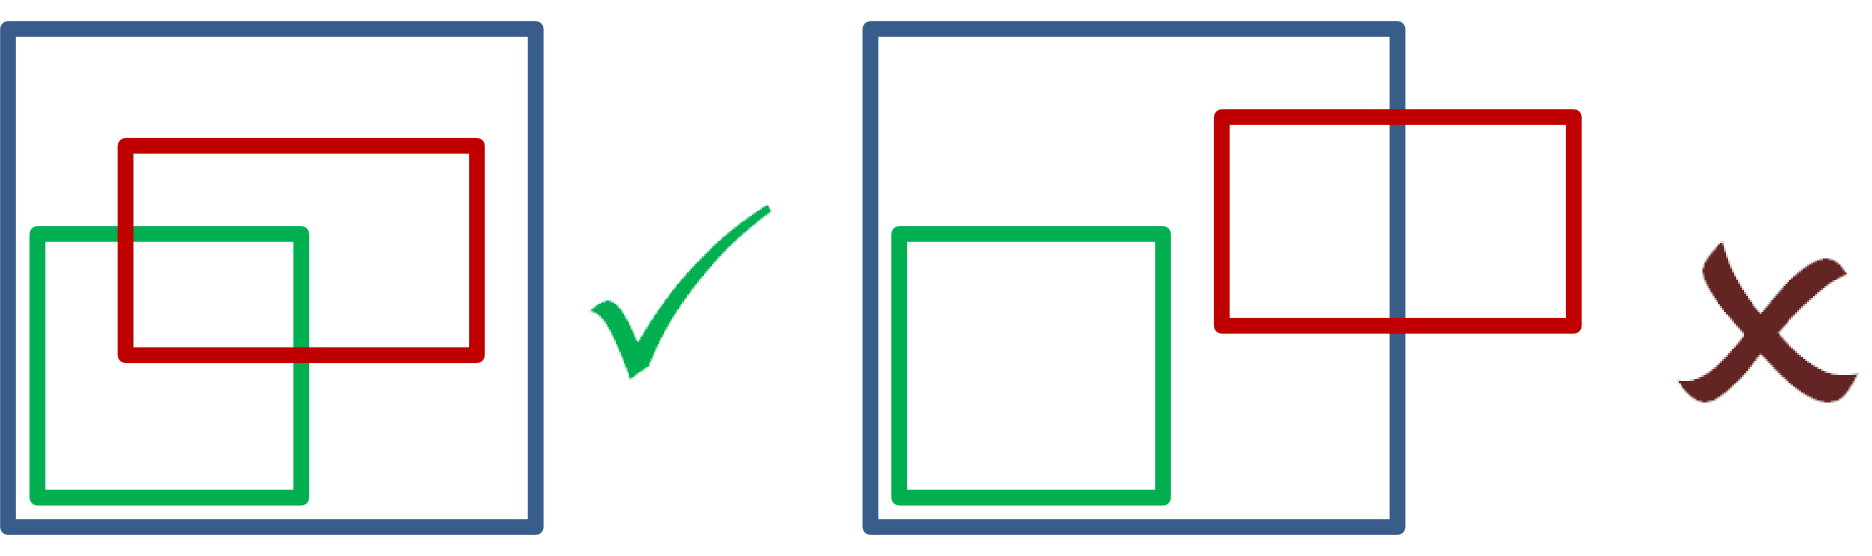
\includegraphics[scale=0.5]{images/post_processing_nested.png}
  \caption{Verschachtelte Semantic Change Sets}
  \label{fig:post_processing_nested}
\end{figure}

Diese Situation lässt sich auch ganz gut aus Sicht der Regeln betrachten. Ist das Metamodell
vollständig durch Atomic-Regeln abgedeckt, dann sollten sich alle Advanced-Regeln in Atomic-Regeln
zerlegen lassen. Für die verbliebenen SCS heißt das, dass bei genau solchen Fällen alle SCS, die
durch Atomic-Regeln entstanden sind, verworfen werden und nur die SCS erhalten bleiben, die durch
die überdeckenden Advanced-Regeln entstanden sind. Problematisch sind dann nur noch sich überschneidende
SCS, die durch Advanced-Regeln erzeugt wurden. Solche Zusammensetzungen können an dieser Stelle noch
nicht gelöst werden. Damit verbleiben alle SCS in der Differenz, die sich in Teilbereichen
überschneiden, aber auch alle SCS, die in solche SCS verschachtelt sind.

\section{Semantic Change Sets mit exklusiven low-level Änderungen}

Nach der Überschneidungsfreiheit der SCS ist die Forderung nach einer möglichst guten Abdeckung
aller low-level Änderungen das nächst wichtigere Optimierungskriterium. Ist in $PCS_D$ zu diesem
Zeitpunkt ein SCS \textit{X} vorhanden, das low-level Änderungen enthält, die in keinem anderen SCS
enthalten sind, dann müsste SCS \textit{X} grundsätzlich in $PCS_{min}$ übernommen werden, um eine
vollständige Abdeckung aller low-level Änderungen zu erreichen. Dies gilt allerdings nur dann, wenn
alle mit SCS \textit{X} überlappenden SCS aus $PCS_D$ entfernt werden können, ohne ungruppierte
low-level Änderungen zu erzeugen. Ansonsten kann diese Operation für SCS \textit{X} nicht ausgeführt
werden, da hier noch nicht entschieden werden kann, ob es nicht evtl. eine bessere Kombination von
SCS gibt, durch die weniger ungruppierte low-level Änderungen entstehen. 

Vorausgesetzt alle Korrespondenzen wurden korrekt ermittelt (Abschintt \ref{sec:matching} Matching),
ist ein solcher Fall wie hier beschrieben ein Indiz dafür, dass die Atomic-Regelbasis nicht
vollständig ist, da sonst beim Entfernen eines überlappenden SCS die restlichen low-level Änderungen
immer maximal in SCS zerfallen, die von Atomic-Regeln stammen.

\begin{figure}[htb]
  \centering
  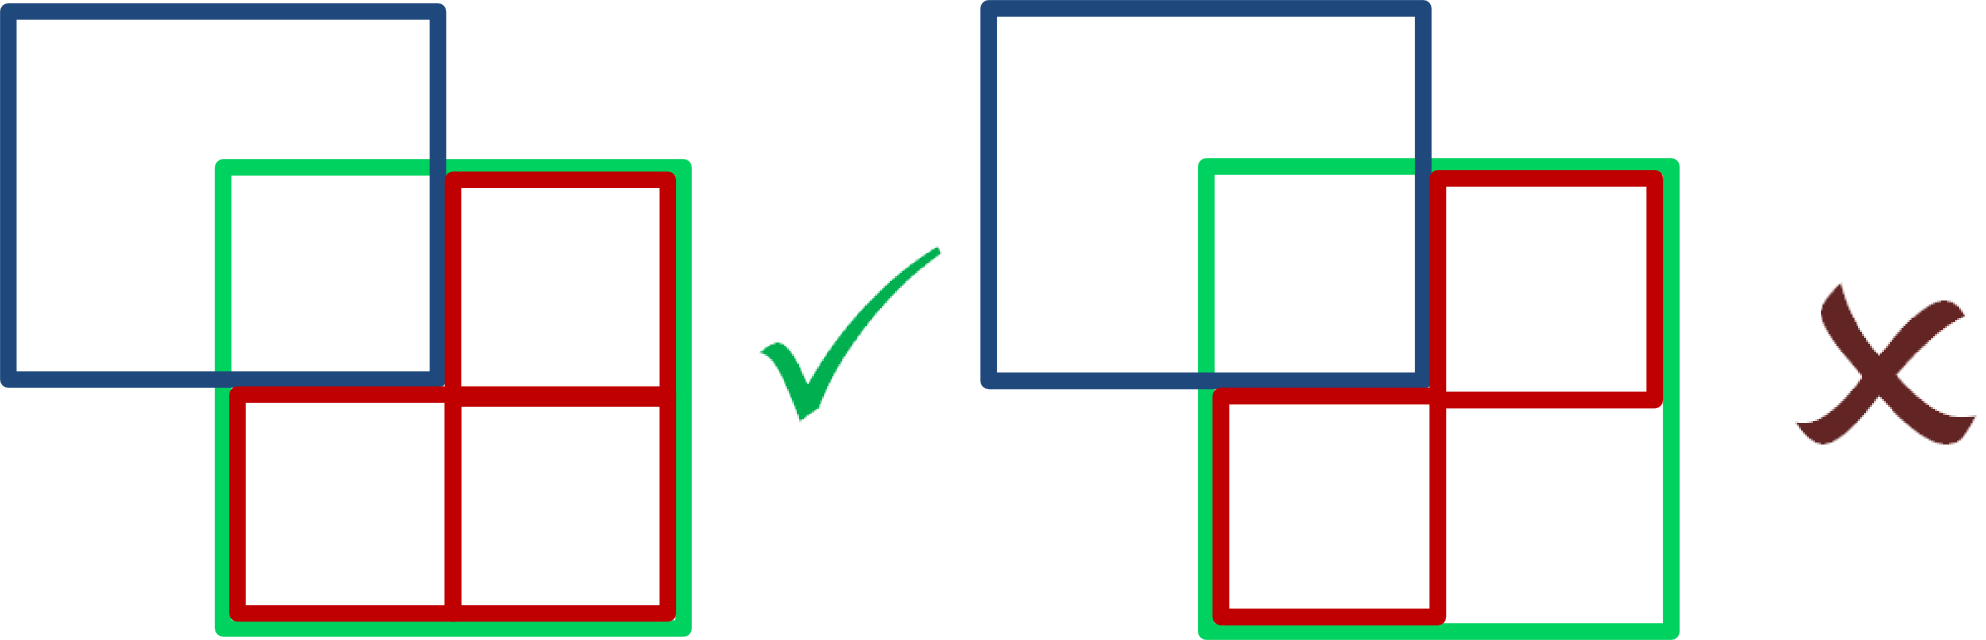
\includegraphics[scale=0.5]{images/post_processing_exclusive.png}
  \caption{Semantic Change Sets mit exklusiven low-level Änderungen}
  \label{fig:post_processing_exclusive}
\end{figure}

\section{Minimierung der Semantic Change Set Menge}

Alle SCS, die jetzt noch in $PCS_D$ enthalten sind, überschneiden sich so, dass sich nicht sofort
eindeutig feststellen lässt, welche Kombination zu einem optimalen Ergebnis führt. Daher werden alle
möglichen Kombinationen betrachtet und die beste Kombination ausgewählt. Da die Laufzeit und
Skalierbarkeit eines solchen kombinatorischen Optimierungsproblems stark von der Anzahl der sich
überschneidenden SCS abhängt, werden zunächst alle SCS in $PCS_D$ in disjunkte Mengen zerlegt. D.h
es werden immer nur SCS betrachtet welche durch Überschneidungen eine zusammenhängende Teilmenge von
$PCS_D$ bilden. Eine solche Teilmenge (\textit{engl. subset}) aus $PCS_D$ wird im Folgenden
allgemein als $PCS_{DS}$ bezeichnet. Wobei $PCS_{DS} \subseteq PCS_D$ gilt. In der Praxis kann man
davon ausgehen, dass die $PCS_{DS}$ Teilmengen relativ klein sind.
\begin{quote}
"`Finally, the remaining change sets are partially overlapping. Our practical evaluation has shown
that these cases are very rare."' \cite{KeKT2011ASE} (S.8)
\end{quote}
In der Regel dürfte es daher möglich sein, alle Kombinationen zu berechnen und jede Kombination nach
den genannten Optimierungskriterien zu bewerten. Da keine Abhängigkeit zwischen den einzelnen $PCS_{DS}$
Teilmengen besteht, können alle Teilmengen parallel berechnet werden.

\begin{figure}[htb]
  \centering
  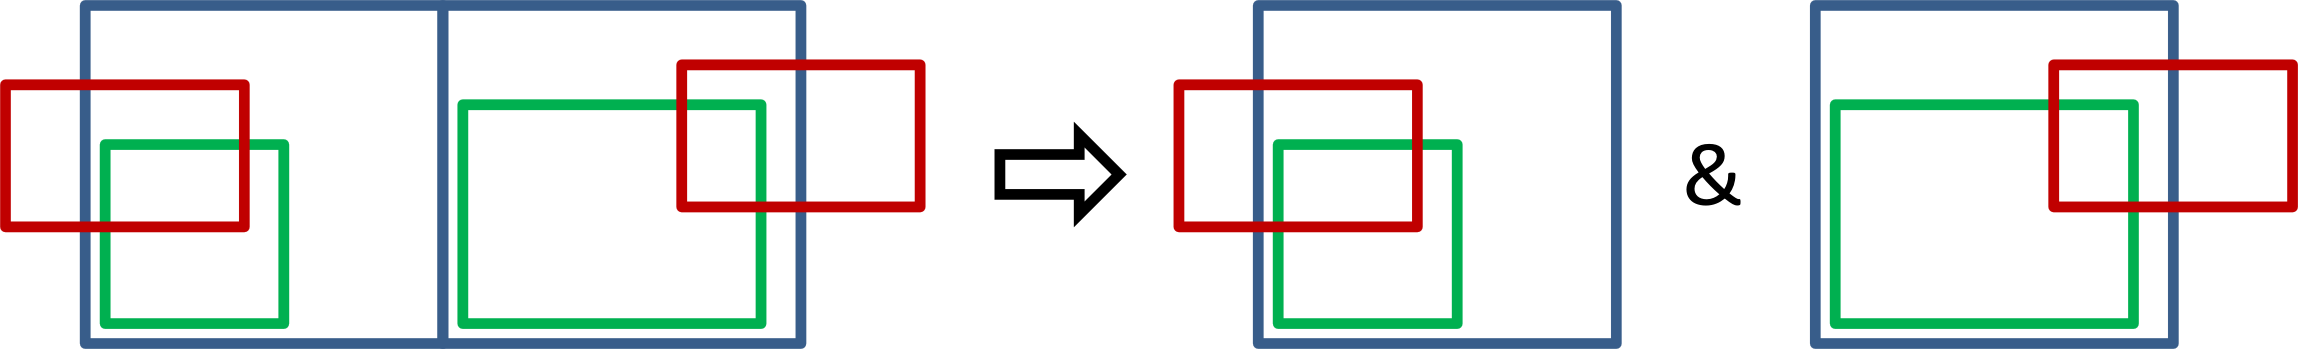
\includegraphics[width=1.0\textwidth]{images/post_processing_disjoint.png}
  \caption{Zerlegung der Semantic-Change-Sets in disjunkte Mengen}
  \label{post_processing_disjoint}
\end{figure}

Sei $PCS_{DS1}$ eine solche Teilmenge aus $PCS_D$. Beim Auswählen der Kombinationen aus $PCS_{DS1}$
spielt die Reihenfolge der SCS innerhalb einer Kombination keine Rolle. Es sollen alle möglichen
Kombinationen ausgewählt werden. Dies entspricht genau der Potenzmenge von $PCS_{DS1}$. Die
Potenzmenge enthält alle möglichen Teilmengen von $PCS_{DS1}$. Bei $n$ SCS in $PCS_{DS1}$ sind dies
genau $2^n$ Teilmengen bzw. Kombinationen, wobei die leere Menge und die Kombination die gleich
$PCS_{DS1}$ ist, vernachlässigt werden können. Damit lässt sich die Komplexität dieses Algorithmus
Schritts bei $n$ SCS pro $PCS_{DS}$ mit $\mathcal{O}(2^n)$ angeben. Das Limit der maximal zu
berechnenden Kombinationen von SCS pro $PCS_{DS}$ kann für das Post-Processing Modul konfiguriert
werden. Ist $(2^n) > Limit$, dann wird die Berechnung der Kombinationen bei Erreichen des Limits
abgebrochen. 

Die Potenzmenge von $PCS_{DS}$ lässt sich relativ leicht über Binärzahlen berechnen. Dazu berechnet
man alle Binärzahlen zwischen $0$ und $2^n$. Durch jede dieser Binärzahlen wird jetzt eine Teilmenge
für die Potenzmenge gebildet, wobei jede Stelle einer Binärzahl mit dem SCS an der entsprechenden
Stelle in $PCS_{DS}$ assoziiert wird. Bei einer 1 wird das SCS in die Teilmenge übernommen und
bei einer 0 nicht. 

\begin{quote}
Zum Beispiel: $PCS_{DS1} = \{SCS1, SCS2, SCS3\}$, $3_d \rightarrow 011_b \Rightarrow \{SCS2, SCS3\}$
\end{quote}

Jede Kombination, die für eine $PCS_{DS}$ Teilmenge berechnet wird muss anschließend bewertet
werden. Alle Kombinationen, die überlappende SCS enthalten, können dabei übersprungen werden. Für
das wichtigste Kriterium wird zunächst die Anzahl der low-level Änderungen bestimmt, welche in den SCS
von $PCS_{DS}$, aber nicht in den SCS der Kombination enthalten sind. Dies sind genau die low-level
Änderungen, die später ungruppiert wären, wenn diese Kombination als beste Lösung für das Problem
ausgewählt würde. Es werden immer die Kombinationen bevorzugt, welche am wenigsten ungruppierte
low-level Änderungen produzieren. Das nächst wichtigere Kriterium ist eine möglichst große
Kompression der Differenz zu erhalten. Die Kompression ergibt sich in diesem Fall aus der Anzahl der
SCS in der Kombination zur Anzahl der SCS in $PCS_{DS}$. Für den Vergleich der Kombinationen heißt
dies, dass immer die Kombination mit den wenigsten SCS bevorzugt wird. Wobei zu beachten ist, dass
die Kompression erst dann verglichen wird, wenn die Anzahl der ungruppierten low-level Änderungen
der Kombinationen gleich ist. Die beste Kombination, die jeweils für eine $PCS_{DS}$ Teilmenge
gefunden wurde, wird dann in $PCS_{min}$ übernommen und alle $PCS_{DS}$ werden aus $PCS_D$ entfernt.

\section{Ergebnis}

Damit ist $PCS_D$ leer. Alle SCS, die nun in $PCS_{min}$ sind, bleiben in der Differenz erhalten und
alle anderen werden entfernt. ($Differenz = Differenz \bigcap PCS_{min}$)  Im Idealfall wurden
durch das Post-Processing keine ungruppierten SCS erzeugt. Entstehen ungruppierte SCS, kann das ein
Indiz dafür sein, dass die Atomic-Regelbasis nicht vollständig ist oder dass nicht korrekte Korrespondenzen
gebildet wurden. Auf jeden Fall muss die Differenz nach dem Post-Processing überschneidungsfrei
sein.
